% Created by tikzDevice version 0.10.1 on 2016-08-26 09:49:51
% !TEX encoding = UTF-8 Unicode
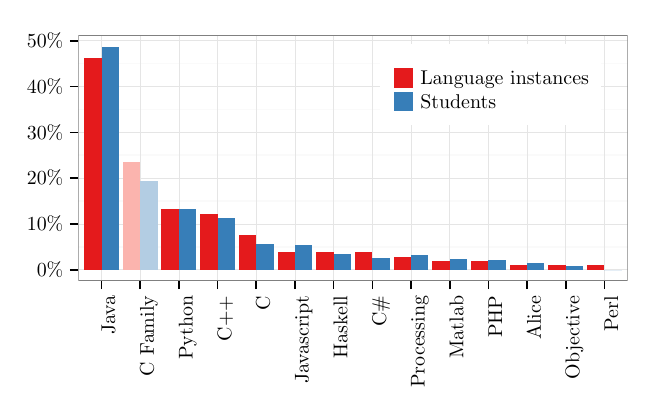
\begin{tikzpicture}[x=1pt,y=1pt]
\definecolor{fillColor}{RGB}{255,255,255}
\path[use as bounding box,fill=fillColor,fill opacity=0.00] (0,0) rectangle (216.81,130.09);
\begin{scope}
\path[clip] (  0.00,  0.00) rectangle (216.81,130.09);
\definecolor{drawColor}{RGB}{255,255,255}
\definecolor{fillColor}{RGB}{255,255,255}

\path[draw=drawColor,line width= 0.6pt,line join=round,line cap=round,fill=fillColor] (  0.00,  0.00) rectangle (216.81,130.09);
\end{scope}
\begin{scope}
\path[clip] ( 18.29, 38.59) rectangle (216.81,127.24);
\definecolor{fillColor}{RGB}{255,255,255}

\path[fill=fillColor] ( 18.29, 38.59) rectangle (216.81,127.24);
\definecolor{drawColor}{gray}{0.98}

\path[draw=drawColor,line width= 0.6pt,line join=round] ( 18.29, 50.90) --
	(216.81, 50.90);

\path[draw=drawColor,line width= 0.6pt,line join=round] ( 18.29, 67.45) --
	(216.81, 67.45);

\path[draw=drawColor,line width= 0.6pt,line join=round] ( 18.29, 84.00) --
	(216.81, 84.00);

\path[draw=drawColor,line width= 0.6pt,line join=round] ( 18.29,100.55) --
	(216.81,100.55);

\path[draw=drawColor,line width= 0.6pt,line join=round] ( 18.29,117.09) --
	(216.81,117.09);
\definecolor{drawColor}{gray}{0.90}

\path[draw=drawColor,line width= 0.2pt,line join=round] ( 18.29, 42.62) --
	(216.81, 42.62);

\path[draw=drawColor,line width= 0.2pt,line join=round] ( 18.29, 59.17) --
	(216.81, 59.17);

\path[draw=drawColor,line width= 0.2pt,line join=round] ( 18.29, 75.72) --
	(216.81, 75.72);

\path[draw=drawColor,line width= 0.2pt,line join=round] ( 18.29, 92.27) --
	(216.81, 92.27);

\path[draw=drawColor,line width= 0.2pt,line join=round] ( 18.29,108.82) --
	(216.81,108.82);

\path[draw=drawColor,line width= 0.2pt,line join=round] ( 18.29,125.37) --
	(216.81,125.37);

\path[draw=drawColor,line width= 0.2pt,line join=round] ( 26.68, 38.59) --
	( 26.68,127.24);

\path[draw=drawColor,line width= 0.2pt,line join=round] ( 40.66, 38.59) --
	( 40.66,127.24);

\path[draw=drawColor,line width= 0.2pt,line join=round] ( 54.64, 38.59) --
	( 54.64,127.24);

\path[draw=drawColor,line width= 0.2pt,line join=round] ( 68.62, 38.59) --
	( 68.62,127.24);

\path[draw=drawColor,line width= 0.2pt,line join=round] ( 82.60, 38.59) --
	( 82.60,127.24);

\path[draw=drawColor,line width= 0.2pt,line join=round] ( 96.58, 38.59) --
	( 96.58,127.24);

\path[draw=drawColor,line width= 0.2pt,line join=round] (110.56, 38.59) --
	(110.56,127.24);

\path[draw=drawColor,line width= 0.2pt,line join=round] (124.54, 38.59) --
	(124.54,127.24);

\path[draw=drawColor,line width= 0.2pt,line join=round] (138.52, 38.59) --
	(138.52,127.24);

\path[draw=drawColor,line width= 0.2pt,line join=round] (152.50, 38.59) --
	(152.50,127.24);

\path[draw=drawColor,line width= 0.2pt,line join=round] (166.48, 38.59) --
	(166.48,127.24);

\path[draw=drawColor,line width= 0.2pt,line join=round] (180.46, 38.59) --
	(180.46,127.24);

\path[draw=drawColor,line width= 0.2pt,line join=round] (194.44, 38.59) --
	(194.44,127.24);

\path[draw=drawColor,line width= 0.2pt,line join=round] (208.42, 38.59) --
	(208.42,127.24);
\definecolor{fillColor}{RGB}{228,26,28}

\path[fill=fillColor] ( 20.39, 42.62) rectangle ( 26.68,119.12);
\definecolor{fillColor}{RGB}{55,126,184}

\path[fill=fillColor] ( 26.68, 42.62) rectangle ( 32.97,123.21);
\definecolor{fillColor}{RGB}{251,180,174}

\path[fill=fillColor] ( 34.37, 42.62) rectangle ( 40.66, 81.65);
\definecolor{fillColor}{RGB}{179,205,227}

\path[fill=fillColor] ( 40.66, 42.62) rectangle ( 46.95, 74.83);
\definecolor{fillColor}{RGB}{228,26,28}

\path[fill=fillColor] ( 48.35, 42.62) rectangle ( 54.64, 64.48);
\definecolor{fillColor}{RGB}{55,126,184}

\path[fill=fillColor] ( 54.64, 42.62) rectangle ( 60.93, 64.53);
\definecolor{fillColor}{RGB}{228,26,28}

\path[fill=fillColor] ( 62.33, 42.62) rectangle ( 68.62, 62.92);
\definecolor{fillColor}{RGB}{55,126,184}

\path[fill=fillColor] ( 68.62, 42.62) rectangle ( 74.91, 61.42);
\definecolor{fillColor}{RGB}{228,26,28}

\path[fill=fillColor] ( 76.31, 42.62) rectangle ( 82.60, 55.11);
\definecolor{fillColor}{RGB}{55,126,184}

\path[fill=fillColor] ( 82.60, 42.62) rectangle ( 88.89, 51.84);
\definecolor{fillColor}{RGB}{228,26,28}

\path[fill=fillColor] ( 90.29, 42.62) rectangle ( 96.58, 48.87);
\definecolor{fillColor}{RGB}{55,126,184}

\path[fill=fillColor] ( 96.58, 42.62) rectangle (102.87, 51.42);
\definecolor{fillColor}{RGB}{228,26,28}

\path[fill=fillColor] (104.27, 42.62) rectangle (110.56, 48.87);
\definecolor{fillColor}{RGB}{55,126,184}

\path[fill=fillColor] (110.56, 42.62) rectangle (116.85, 48.32);
\definecolor{fillColor}{RGB}{228,26,28}

\path[fill=fillColor] (118.25, 42.62) rectangle (124.54, 48.87);
\definecolor{fillColor}{RGB}{55,126,184}

\path[fill=fillColor] (124.54, 42.62) rectangle (130.83, 46.82);
\definecolor{fillColor}{RGB}{228,26,28}

\path[fill=fillColor] (132.23, 42.62) rectangle (138.52, 47.31);
\definecolor{fillColor}{RGB}{55,126,184}

\path[fill=fillColor] (138.52, 42.62) rectangle (144.81, 47.95);
\definecolor{fillColor}{RGB}{228,26,28}

\path[fill=fillColor] (146.21, 42.62) rectangle (152.50, 45.74);
\definecolor{fillColor}{RGB}{55,126,184}

\path[fill=fillColor] (152.50, 42.62) rectangle (158.79, 46.60);
\definecolor{fillColor}{RGB}{228,26,28}

\path[fill=fillColor] (160.19, 42.62) rectangle (166.48, 45.74);
\definecolor{fillColor}{RGB}{55,126,184}

\path[fill=fillColor] (166.48, 42.62) rectangle (172.77, 46.14);
\definecolor{fillColor}{RGB}{228,26,28}

\path[fill=fillColor] (174.17, 42.62) rectangle (180.46, 44.18);
\definecolor{fillColor}{RGB}{55,126,184}

\path[fill=fillColor] (180.46, 42.62) rectangle (186.75, 44.88);
\definecolor{fillColor}{RGB}{228,26,28}

\path[fill=fillColor] (188.15, 42.62) rectangle (194.44, 44.18);
\definecolor{fillColor}{RGB}{55,126,184}

\path[fill=fillColor] (194.44, 42.62) rectangle (200.73, 43.83);
\definecolor{fillColor}{RGB}{228,26,28}

\path[fill=fillColor] (202.13, 42.62) rectangle (208.42, 44.18);
\definecolor{fillColor}{RGB}{55,126,184}

\path[fill=fillColor] (208.42, 42.62) rectangle (214.71, 42.62);
\definecolor{drawColor}{gray}{0.50}

\path[draw=drawColor,line width= 0.6pt,line join=round,line cap=round] ( 18.29, 38.59) rectangle (216.81,127.24);
\end{scope}
\begin{scope}
\path[clip] (  0.00,  0.00) rectangle (216.81,130.09);
\definecolor{drawColor}{RGB}{0,0,0}

\node[text=drawColor,anchor=base east,inner sep=0pt, outer sep=0pt, scale=  0.72] at ( 12.89, 40.14) {0\%};

\node[text=drawColor,anchor=base east,inner sep=0pt, outer sep=0pt, scale=  0.72] at ( 12.89, 56.69) {10\%};

\node[text=drawColor,anchor=base east,inner sep=0pt, outer sep=0pt, scale=  0.72] at ( 12.89, 73.24) {20\%};

\node[text=drawColor,anchor=base east,inner sep=0pt, outer sep=0pt, scale=  0.72] at ( 12.89, 89.79) {30\%};

\node[text=drawColor,anchor=base east,inner sep=0pt, outer sep=0pt, scale=  0.72] at ( 12.89,106.34) {40\%};

\node[text=drawColor,anchor=base east,inner sep=0pt, outer sep=0pt, scale=  0.72] at ( 12.89,122.89) {50\%};
\end{scope}
\begin{scope}
\path[clip] (  0.00,  0.00) rectangle (216.81,130.09);
\definecolor{drawColor}{RGB}{0,0,0}

\path[draw=drawColor,line width= 0.6pt,line join=round] ( 15.29, 42.62) --
	( 18.29, 42.62);

\path[draw=drawColor,line width= 0.6pt,line join=round] ( 15.29, 59.17) --
	( 18.29, 59.17);

\path[draw=drawColor,line width= 0.6pt,line join=round] ( 15.29, 75.72) --
	( 18.29, 75.72);

\path[draw=drawColor,line width= 0.6pt,line join=round] ( 15.29, 92.27) --
	( 18.29, 92.27);

\path[draw=drawColor,line width= 0.6pt,line join=round] ( 15.29,108.82) --
	( 18.29,108.82);

\path[draw=drawColor,line width= 0.6pt,line join=round] ( 15.29,125.37) --
	( 18.29,125.37);
\end{scope}
\begin{scope}
\path[clip] (  0.00,  0.00) rectangle (216.81,130.09);
\definecolor{drawColor}{RGB}{0,0,0}

\path[draw=drawColor,line width= 0.6pt,line join=round] ( 26.68, 35.59) --
	( 26.68, 38.59);

\path[draw=drawColor,line width= 0.6pt,line join=round] ( 40.66, 35.59) --
	( 40.66, 38.59);

\path[draw=drawColor,line width= 0.6pt,line join=round] ( 54.64, 35.59) --
	( 54.64, 38.59);

\path[draw=drawColor,line width= 0.6pt,line join=round] ( 68.62, 35.59) --
	( 68.62, 38.59);

\path[draw=drawColor,line width= 0.6pt,line join=round] ( 82.60, 35.59) --
	( 82.60, 38.59);

\path[draw=drawColor,line width= 0.6pt,line join=round] ( 96.58, 35.59) --
	( 96.58, 38.59);

\path[draw=drawColor,line width= 0.6pt,line join=round] (110.56, 35.59) --
	(110.56, 38.59);

\path[draw=drawColor,line width= 0.6pt,line join=round] (124.54, 35.59) --
	(124.54, 38.59);

\path[draw=drawColor,line width= 0.6pt,line join=round] (138.52, 35.59) --
	(138.52, 38.59);

\path[draw=drawColor,line width= 0.6pt,line join=round] (152.50, 35.59) --
	(152.50, 38.59);

\path[draw=drawColor,line width= 0.6pt,line join=round] (166.48, 35.59) --
	(166.48, 38.59);

\path[draw=drawColor,line width= 0.6pt,line join=round] (180.46, 35.59) --
	(180.46, 38.59);

\path[draw=drawColor,line width= 0.6pt,line join=round] (194.44, 35.59) --
	(194.44, 38.59);

\path[draw=drawColor,line width= 0.6pt,line join=round] (208.42, 35.59) --
	(208.42, 38.59);
\end{scope}
\begin{scope}
\path[clip] (  0.00,  0.00) rectangle (216.81,130.09);
\definecolor{drawColor}{RGB}{0,0,0}

\node[text=drawColor,rotate= 90.00,anchor=base east,inner sep=0pt, outer sep=0pt, scale=  0.72] at ( 31.64, 33.19) {Java};

\node[text=drawColor,rotate= 90.00,anchor=base east,inner sep=0pt, outer sep=0pt, scale=  0.72] at ( 45.62, 33.19) {C Family};

\node[text=drawColor,rotate= 90.00,anchor=base east,inner sep=0pt, outer sep=0pt, scale=  0.72] at ( 59.60, 33.19) {Python};

\node[text=drawColor,rotate= 90.00,anchor=base east,inner sep=0pt, outer sep=0pt, scale=  0.72] at ( 73.58, 33.19) {C++};

\node[text=drawColor,rotate= 90.00,anchor=base east,inner sep=0pt, outer sep=0pt, scale=  0.72] at ( 87.56, 33.19) {C};

\node[text=drawColor,rotate= 90.00,anchor=base east,inner sep=0pt, outer sep=0pt, scale=  0.72] at (101.54, 33.19) {Javascript};

\node[text=drawColor,rotate= 90.00,anchor=base east,inner sep=0pt, outer sep=0pt, scale=  0.72] at (115.52, 33.19) {Haskell};

\node[text=drawColor,rotate= 90.00,anchor=base east,inner sep=0pt, outer sep=0pt, scale=  0.72] at (129.50, 33.19) {C\#};

\node[text=drawColor,rotate= 90.00,anchor=base east,inner sep=0pt, outer sep=0pt, scale=  0.72] at (143.48, 33.19) {Processing};

\node[text=drawColor,rotate= 90.00,anchor=base east,inner sep=0pt, outer sep=0pt, scale=  0.72] at (157.46, 33.19) {Matlab};

\node[text=drawColor,rotate= 90.00,anchor=base east,inner sep=0pt, outer sep=0pt, scale=  0.72] at (171.44, 33.19) {PHP};

\node[text=drawColor,rotate= 90.00,anchor=base east,inner sep=0pt, outer sep=0pt, scale=  0.72] at (185.42, 33.19) {Alice};

\node[text=drawColor,rotate= 90.00,anchor=base east,inner sep=0pt, outer sep=0pt, scale=  0.72] at (199.40, 33.19) {Objective};

\node[text=drawColor,rotate= 90.00,anchor=base east,inner sep=0pt, outer sep=0pt, scale=  0.72] at (213.38, 33.19) {Perl};
\end{scope}
\begin{scope}
\path[clip] (  0.00,  0.00) rectangle (216.81,130.09);
\definecolor{fillColor}{RGB}{255,255,255}

\path[fill=fillColor] (127.26, 94.90) rectangle (207.10,124.12);
\end{scope}
\begin{scope}
\path[clip] (  0.00,  0.00) rectangle (216.81,130.09);
\definecolor{fillColor}{RGB}{228,26,28}

\path[fill=fillColor] (132.24,108.42) rectangle (139.35,115.53);
\end{scope}
\begin{scope}
\path[clip] (  0.00,  0.00) rectangle (216.81,130.09);
\definecolor{fillColor}{RGB}{55,126,184}

\path[fill=fillColor] (132.24, 99.88) rectangle (139.35,106.99);
\end{scope}
\begin{scope}
\path[clip] (  0.00,  0.00) rectangle (216.81,130.09);
\definecolor{drawColor}{RGB}{0,0,0}

\node[text=drawColor,anchor=base west,inner sep=0pt, outer sep=0pt, scale=  0.72] at (141.87,109.49) {Language instances};
\end{scope}
\begin{scope}
\path[clip] (  0.00,  0.00) rectangle (216.81,130.09);
\definecolor{drawColor}{RGB}{0,0,0}

\node[text=drawColor,anchor=base west,inner sep=0pt, outer sep=0pt, scale=  0.72] at (141.87,100.96) {Students};
\end{scope}
\end{tikzpicture}
